\section{Introduzione}

\textcolor{blue}{\lipsum[1-2]}

\section{Background}

Un sistema di controllo è un apparato che consente di variare o mantenere constanti le grandezze di uscita in relazione ad un'evoluzione temporale delle grandezze di ingresso. Ovvero, un insieme di componenti interconnessi che lavorano per raggiungere una determinata risposta anche in presenza di stimoli esterni \cite{marro_controlli_2004}.  

Si parla di regolazione, o controllo semplice, quando si richiede che l'uscita rimanga costante al variare dell'ingresso.

Ove possibile si utilizzano sistemi di controllo ad anello chiuso dove si identifica anche il blocco di retroazione che genera un segnale proporzione al valore della grandezza controllata, riportandolo in ingresso al controllore.

All'interno degli organismi biologici si trovano diversi sistemi di controllo, più o meno complessi, alcuni locali e altri diffusi su tutto l'organismo, volti a mantenere l'omeostasi dell'organismo. 

Il termine omeostasi fu introdotto nel 1865 da Claude Bernard per rappresentare come l'organismo cercasse di mantenere costante l'ambiente interno del corpo \cite{bernard1957introduction}. Il termine fu poi coniato da Walter Bradford Cannon, ampliandone il significato e introducendo il fatto che l'omeostasi non è uno stato statico stazionario ma è un proprio un continuo evolversi di stati di equilibrio e di condizioni che possono continuamente variare \cite{cannon1939wisdom}. Questo è dovuto all'elevata complessità dei sistemi di controllo fisiologici che coinvolgono sicuramente il sistema nervoso ma anche i singoli organi. 

Quindi, l'estensione del concetto di omeostasi può essere visto come l'oscillazione nel tempo intorno ad un valore medio caratteristico di ogni variabile fisiologica. Tale oscillazione nel tempo può essere riferita a secondi, minuti, giorni, ore o anni a secondi di quale parametro si considera. Tuttavia, trascorriamo la maggior parte del tempo oscillando tra un valore massimo e minimo, attorno al valore medio, in un range considerato normale. Tale range è proprio ciò che viene definito omeostasi \cite{davies_adaptive_2016}. 



\subsection{Riflesso neuromuscolare}

Quando un muscolo intero viene stirato passivamente le fibre del fuso neuromuscolare si stirano e uamentnao la frequenza di scarica nelle fibre nervose afferenti. Le loro terminazioni sensnoriali terminano sulle lifbre intrafusai stirale e il neurore afferente stabilisce contatti sinaptici direttamente sul motoneurone $\alpha$ che innerva le fibre extrafusali dello stesso muscolo determinanone la contrazione. 

Questo riflesso miotatico funge da meccnaismo locale a feedback negativo che permette di opporsi ad ogni variazione passiva della lunghezza muscolare, cos'ì da mantenere la lungezza di stiramento ottimale. 

Ne sono esempi il riflesso rotuleo o il riflesso da stiramento nel bracciom entrambi usati anche come test di routine per valutare il sisitema nervoso. 

Tali riflessi possono essere assenti o depressi a causa di perdite di input eccitatori dai livelli supeiori o per perdite di input inibitori ai motoneuroni dai livelli encefalici superiorii \cite{sherwood_fisiologia_2008}.

Tale riflesso coinvolge il muscolo stesso, il fuso neuromuscolare e i motoneuroni. Tali partecipanti possono essere rifvisti come un sisitema di controllo. 

Concentrandoci sull'arto superiore è possibile vedere il centro del riflesso nel midollo spinale, dove avviene la sinapsi tra le vie afferenti e i motoneruroni $\alpha$ per regolare il muscolo a seconda del disturbo indotto dal carico.

Un diagramma a blocchi di tale sisitema di controllo è presente in \cref{fig:sistemamuscolo}.

\begin{figure}[t!]
	\centering
	\footnotesize{\def\svgwidth{0.95\linewidth}
	\input{blocchi_stretch.pdf_tex}}
	\caption{Diagramma a blocchi del riflesso neuromuscolare}
	\label{fig:sistemamuscolo}
\end{figure}

Affinchè sia possibile analizzare i singoli sistemi è necessario adottare un modello matematico descrittivo.

Partendo dalla descrizione geoemetrica in \cref{fig:avambraccio} il sisitema è descritto dalla seguente equazione:

\begin{equation}
	M_{x}(t)-M(t)=J \ddot{\theta}
\end{equation}

\begin{figure*}[t!]
	\centering
	\begin{subfigure}{0.7\linewidth}
		\centering
	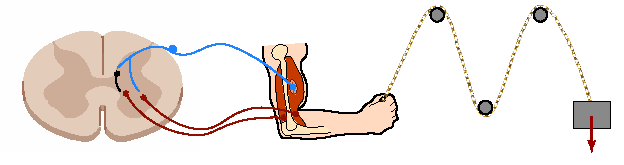
\includegraphics[width=0.95\linewidth]{figures/avambraccio_schema}\caption{}
	\end{subfigure}\hfill
\begin{subfigure}{0.3\linewidth}
	\centering
\footnotesize{\def\svgwidth{0.9\linewidth}
\input{avambraccio_modello.pdf_tex}}
\caption{}
\end{subfigure}
	\caption{Rappresentazione schematica del test diagnostico per il riflesso da stiramento del braccio (a). Il carico viene applicato tramite una carrucola e va stimolare i recettori del fuso neuromuscolare che a loro volta vanno a stimolare i percorsi delle vie riflesse all'interno del canale spinale; gradi di libertà del sistema braccio-avambraccio (b) dove la coppia è esercitata dal muscolo}
	\label{fig:avambraccio}
\end{figure*}

\begin{figure*}[h!]
	\centering
	\begin{subfigure}{0.33\linewidth}
		\centering
		\footnotesize{\def\svgwidth{0.9\linewidth}
			\input{modello_muscolo_schema.pdf_tex}}
		\caption{}
	\end{subfigure}\hfill
\begin{subfigure}{0.33\linewidth}
	\centering
	\tiny{\def\svgwidth{0.8\linewidth}
		\input{fuso_modello.pdf_tex}}
	\caption{}
\end{subfigure}\hfill
	\begin{subfigure}{0.33\linewidth}
	\centering
	\footnotesize{\def\svgwidth{0.9\linewidth}
		\input{modello_fuso_schema.pdf_tex}}
	\caption{}
\end{subfigure}\hfill
	\caption{Modello muscolare di Hill (a); relazione tra muscolo e fuso neuromuscolare (b); modello di fuso neuromuscolare di Soechting (c)}
	\label{fig:fuso}
\end{figure*}





\subsubsection{Modello di muscolo}

Viene considerato il modello di muscolo di Hill \cite{hill_heat_1938}. Tale modello, a parametri concentrati, considera il muscolo come la serie di due zone. La prima zona è data da un parallelo di una coppia motrice (forza muscolare) e uno smorzamento, in serie ad una rigidezza elastica.

Mentre lo spostamento angolare sarà la somma dei due blocchi, la coppia risultante sarà uguale nel parallelo:

\begin{equation}
	\begin{gathered}
		M(t)=K\left(\theta-\theta_{1}\right) \\
		K(t)=M_{0}(t)+B \dot{\theta}_{1}
	\end{gathered}
\end{equation}

Quindi può essere descritto dalla seguente equazione:

\begin{equation}
	M_{x}(t)-M_{0}(t)=\frac{B J}{K} \dddot{\theta}(t)+J \ddot{\theta}(t)+B \dot{\theta}(t)
\end{equation}

E, nel dominio di Laplace, da:

\begin{equation}
	M_{x}(s)-M_{0}(s)=s\left(\frac{B J}{k} s^{2}+J s+B\right)
\end{equation}

\subsubsection{Fuso neuromuscolare}

Per il fuso muscolare viene adottare il modello di Soechting \cite{mains_model_1971} dove il fuso viene differenziato tra la parte interna, del nucleo, e la parte polare.

La variabile di interesse è sempre la coordinata angolare e valgono le seguenti relazioni:

\begin{equation}
	\begin{gathered}
		M_{s}(t)=K_{s s}\left(\theta-\theta_{2}\right) \\
		M_{s}(t)=K_{s p}  \theta_{2}+B_{s} \dot{\theta}_{2}
	\end{gathered}
\end{equation}

\subsubsection{Riflesso}

Per il riflesso sappiamo che conta quanto accade a livello del fuso, ovvero avremo la risposta legata all'allungamento per il tramite di un certo guadagno:

\begin{equation}
	M_{0}(t)=\beta\left(\theta-\theta_{2}\right)
\end{equation}

Da cui si trova l'equazione del sistema:

\begin{equation}
	\small{\dot{M}_{0}(t)+\frac{M_{0}(t)}{\tau}=\beta\left(\dot{\theta}\left(t-T_{D}\right)+\frac{\theta\left(t-T_{D}\right)}{\tau \eta}\right)}
\end{equation}

Dove i due parametri, funzioni delle costanti concentrate, sono:

\begin{equation}
	\tau=\frac{B_{s}}{K_{s s}+K_{s p}} \quad \text { e } \eta=\frac{K_{s s}+K_{s p}}{K_{s p}}
\end{equation}

Passando nel dominio di Laplace possiamo ricavare la coppia agente come:

\begin{equation}
	M_{o}(s)=\beta\left(\frac{s \tau+s / \eta}{s \tau+s}\right) e^{-s T_{D}} \theta(s)
\end{equation}

Per l'implementazione in Simulink vengono considerati dei parametri fisiologici, in \cref{tab:parametriMuscolo} \cite{khoo_physiological_2018,soechting_evaluation_1971}. 

\begin{table}[t!]
	\centering
	\begin{tabular}{|c|c|}
		\hline
		Parametro & Valore \\
		\hline
		\texttt{B} & 2 [Nms] \\
		\hline
		\texttt{J} & 0.1 [kg m\textsuperscript{2}] \\
		\hline
		\texttt{Td} & 0.02 [s] \\
		\hline
		\texttt{beta} & 100 \\
		\hline
		\texttt{eta} & 5 \\
		\hline
		\texttt{k} & 50 [Nm] \\
		\hline
		\texttt{tau} & 1/300 [s] \\
		\hline
	\end{tabular}
	\caption{Parametri del sistema descrittivo del riflesso neuromuscolare}
	\label{tab:parametriMuscolo}
\end{table}


\subsection{Riflesso fotomotore}

Un altro riflesso di grande interesse clinico è il riflesso pupillare, noto anche come riflesso fotomotore. Tale riflesso controlla il diametro della pupilla in risposta all'intensitò della luce che arriva alla retina.

il nervo ottico costituisce la via afferente in quanto percepisce la luce in ingresso, tramite  le cellule ganglieri della retina. L'informazione raggiunge il nucelo pretettate nel mesencefalo superiore e poi il nucelo di Edinger-Westphal. Da qui si dipartono i nervi oculomotori fino ai gangli cicliari e all'invervazione del muscolo costrittore della pupilla \cite{kandel_principles_2021}.

In condizioni fisiologiche, le pupille rispondono entrambe in maniera identica. Il confronto delle risposte asimettriche permette di valutare una lesione.
Ad esempio, una risposta diretta in una pupilla senza risposta consensuale nell'aktra indica un possibiile propblema nella connesione motoria della seconda. Oppure, è possibile avere perdite del riflesso diretto mentre rimane attiva la risposta consensuale. 

\subsubsection{Modello di Stark}

Per l'implementazione viene considerato il modello di Stark \cite{stark_servoanalytic_1957}. Tale modello intepreta il flusso di luce come l'intensità luminosa agente sull'area della pupilla e l'obiettivo del controllore (riflesso pupillare) è proprio quello di mantenere tale flusso costante. Se varia il flusso il sisitema nervoso si attiva per variare l'area della pupilla.

Tale modello contiene molte non linearità ma, linerizzandolo intorno al punto di lavoro, permette di descrivere correttamente la risposta fisiologica \cite{khoo_physiological_2018}.

Il diagramma a blocchi del sisitema è presente in \cref{fig:pupilla}. Si considera quindi un sisitema LTI con una funzione di trasferimento del terzo ordine in serie ad un ritardo con costante di tempo $\tau$. Ovvero la funzioen di trasferimento di anello :

\begin{equation}
	H(s)=\frac{K e^{-s D}}{(1+\tau s)^{3}}
\end{equation}

Dove il guadagno è dato dal prodotto del guadagno della funzione di traferimento del cambiamento d'area e del fattore linearizzato di insentità luminosa (rispetto al quale si è linearizzato il modello), ovvero:

\begin{equation}
	K=I_{\text {ref }} K_{1}
\end{equation}

I parametri del sisitema sono presenti in \cref{tab:pupilla}

\begin{table}[t!]
	\centering
	\begin{tabular}{|c|c|}
		\hline
		Parametro & Valore \\
		\hline
		\texttt{K} & 0.16 \\
		\hline
		\texttt{D} & 0.18 [s] \\
		\hline
		\texttt{tau} & 0.1 [s] \\
		\hline
	\end{tabular}
	\caption{Parametri del sistema linearizzato descrittivo del riflesso pupillare}
	\label{tab:pupilla}
\end{table}


\begin{figure*}[h!]
	\centering
	\begin{subfigure}{0.6\linewidth}
\centering
	\tiny{\def\svgwidth{0.95\linewidth}
	\input{occhio_muscoli.pdf_tex}}
\caption{}
	\end{subfigure}\hfill
	\begin{subfigure}{0.4\linewidth}
	\centering
	\tiny{\def\svgwidth{0.95\linewidth}
		\input{circuito_pupilla.pdf_tex}}
	\caption{}
\end{subfigure}
	\caption{}
	\label{fig:pupilla}
\end{figure*}



\begin{figure}[h!]
	\centering
	\footnotesize{\def\svgwidth{0.95\linewidth}
	\input{blocchi_pupillary.pdf_tex}}
\caption{Diagramma a blocchi del riflesso pupillare linearizzato}
\end{figure}


\subsection{Stabilità}

Per un sistema dinamico uno stato di equilibrio è uno stato in cui il sisitema rimane indefinitamente, in assenza di perturbazioni. Se tale stato di equilibrio è stabile (asintoticamente), ciò permette al sisitema di rimanenerci effettivamente. 

Per un sistema lineare si può parlare di stabilità del sisitema stesso, ed in particolare risulta stabile qualora gli autovalori della matrice dinamica del sistema sono a parte reale negativa \cite{grasselli_sistemi_2008}.

Tale definizione matematica può essere particolarizzata in diversi criteri per analizzare la stabilità del singolo sistema.

Considerando un generico sistema a retroazione di equazione caratteristica:

\begin{equation}
	1+G(s)H(s)=0
			\label{eq:retroazione}
\end{equation}

Dove $G(s)$ è la funzione di trasferimento diretta e $H(s)$ la funzione di trasferimento di retroazione e $G(s)H(s)$ la funzione di trasferimento di anello (\cref{fig:sistema}).

Quindi tale per cui:

\begin{equation}
	Y(1+G H)=G X
\end{equation}

E allora la funzione di trasferimento:

\begin{equation}
	W=\frac{Y}{X}=\frac{G}{1+G H}
\end{equation}


\begin{figure}[t!]
	\centering
	\centering
\footnotesize{\def\svgwidth{0.95\linewidth}
	\input{feedback.pdf_tex}}
	\caption{Generico sistema a feedback negativo dove sono presenti la funzione di trasferimento diretta $G$ e la retroazione $H$ che riporta l'uscita in ingresso con segno invertito}
	\label{fig:sistema}
\end{figure}


Considerando che $G(s)H(s)$ è una funzione razionale fratta con guadagno $K$ (positivo per sisitemi a retroazione negativa), le radici di tale equazione descrivono una curva nel piano $s$ che prende il nome di luogo delle radici. 

\begin{equation}
	G(s)H(s)=K\left.N(s)\over D(s)\right.
\end{equation}

Per avere stabilità si richiede che tutti i poli della funzione di trasferimento siano nella parte sinistra del piano, ovvero a parte reale negativa \cite{marro_controlli_2004}. Tali poli corrispondono agli zeri di \cref{eq:retroazione} ovvero a studiare l'andamento:

\begin{equation}
D(s)+KN(s)=0
\end{equation}




\subsection{Simulink}

Simulink \cite{simulink} è un software sviluppato da MathWorks che fornisce un approccio grafico basato su un ambiente di modellazione che permette all’utente di convertire il problema in una rete di blocchi di funzioni matematiche.

Inoltre, tale ambiente permette l’integrazione con il linguaggio Matlab e le relative funzioni di programmazione.

Tramite Simulink è possibile implementare i modelli considerati aggiungendo diverse features, quali delle dashboard per interagire con i parametri del sistema, utili ad analizzarne il comportamento e la stabilità.

\section{Risultati}
\textcolor{blue}{\lipsum[1-5]}


\subsection{Riflesso neuromuscolare}



\subsection{Riflesso pupillare}

\textcolor{blue}{CERCA QUALCOSA SULLA FREQUENZA DELL'HYPPUS}

\section{Conclusioni}

\textcolor{blue}{\lipsum[1-2]}
\raggedbottom
\pagebreak
\section*{Disponibilità dei dati}

Il materiale è disponibile alla repository online del progetto: \url{https://github.com/mastroalex/reflex}


\raggedbottom
%\pagebreak
\printbibliography[title=Riferimenti]
%\section*{References}

\clearpage
\onecolumn
\section*{Appendice}

\subsection{Blocco \texttt{fcn}}

\subsection{Plot}




